\documentclass[../competing_bandits_with_appendix.tex]{subfiles}
\begin{document}

\section{Supplementary experimental results}
\label{app:expts}

\subsection{Plots for ``Performance In Isolation"}

We present additional plots for Section \ref{sec:isolation}. First, we provide mean reputation trajectories for Uniform and Heavy-Tail MAB instances. Second, we provide trajectories for instantaneous mean rewards, for all three MAB instances.%
\footnote{These trajectories are smoothed via a non-parametric regression.
More concretely, we use this option in $\texttt{ggplot}$:
\url{https://ggplot2.tidyverse.org/reference/geom_smooth.html}.}
In all plots, the shaded area represents 95\% confidence interval.

\begin{center}
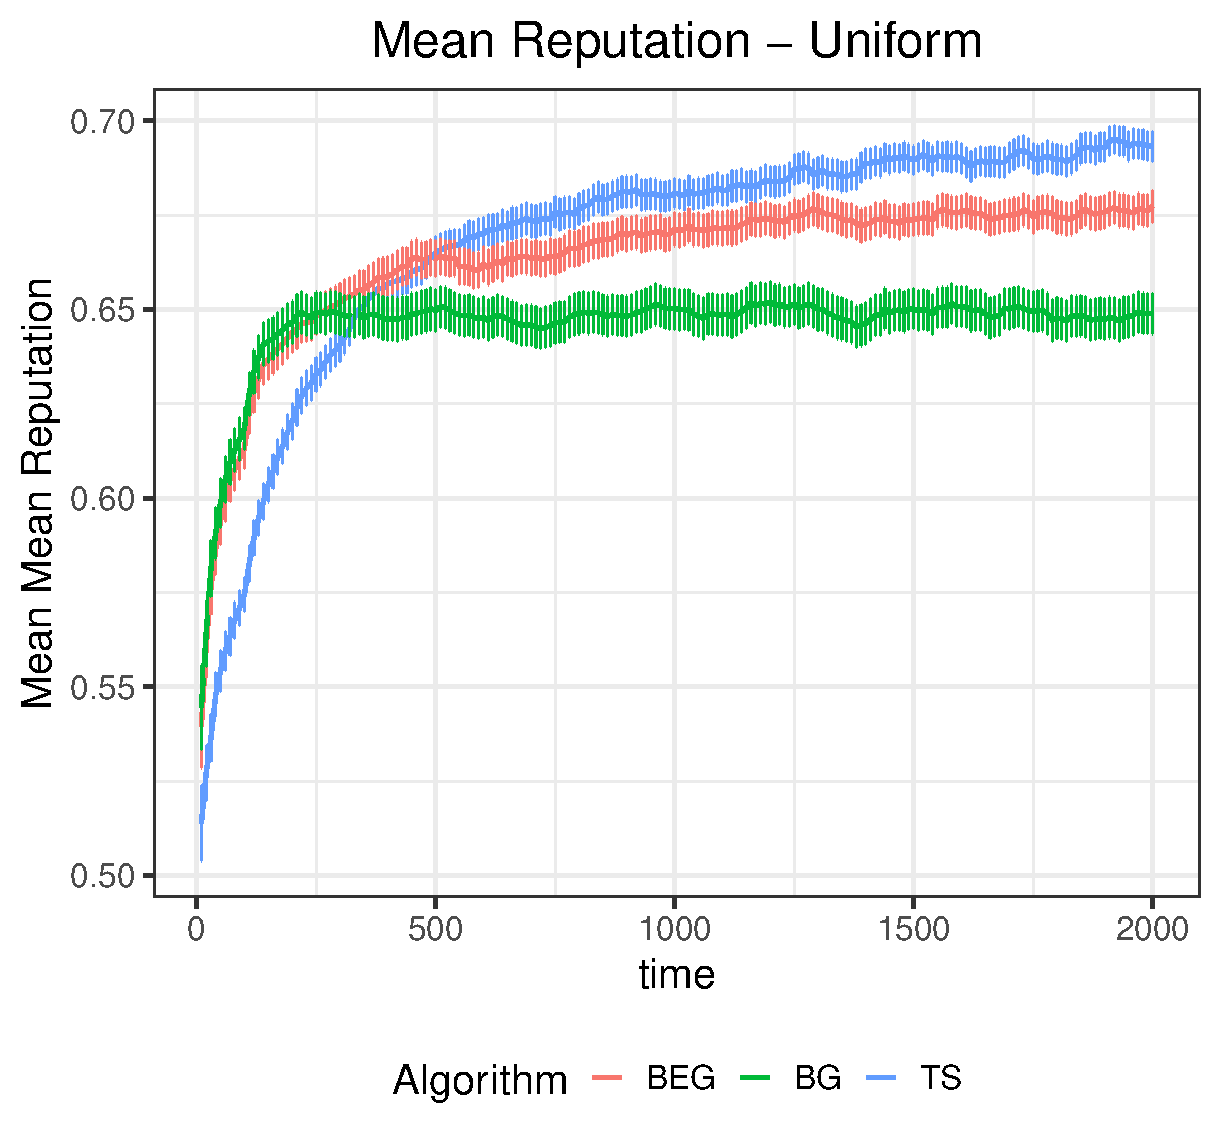
\includegraphics[scale=0.35]{ec19paper/appendix_figures/uniform_mean}
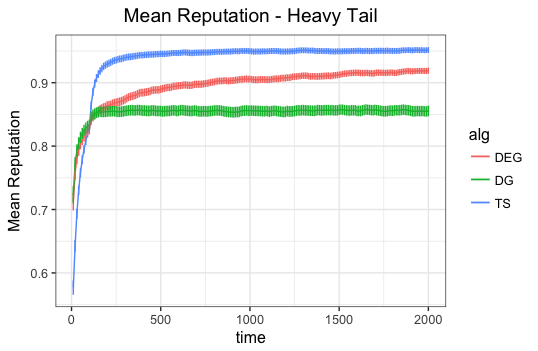
\includegraphics[scale=0.35]{ec19paper/appendix_figures/ht_mean}
\end{center}
\begin{center}
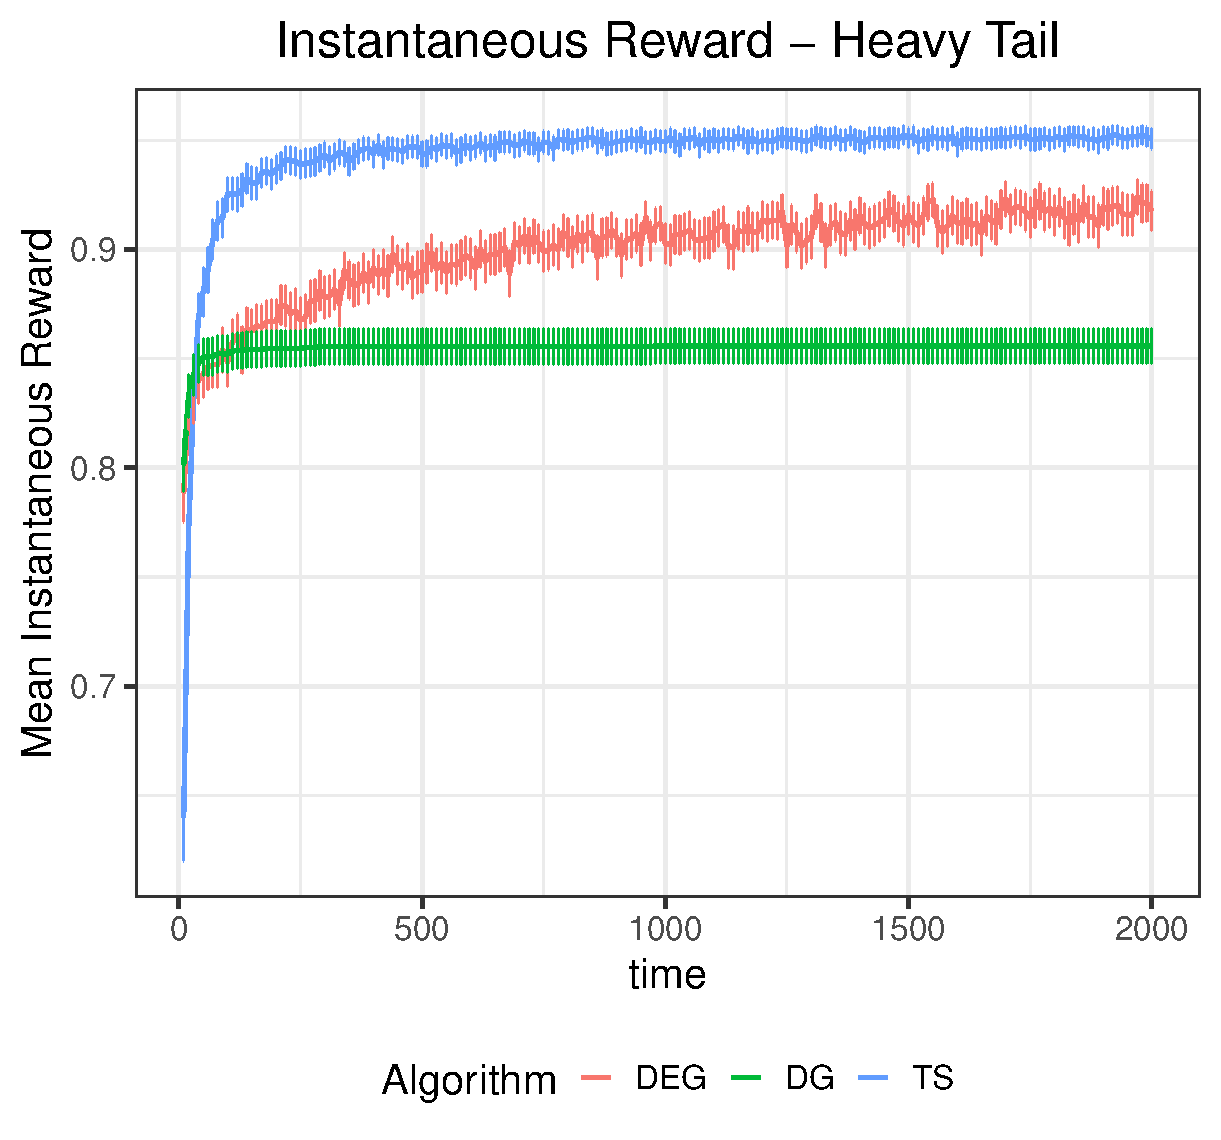
\includegraphics[scale=0.35]{ec19paper/appendix_figures/mean_inst_reward_ht}
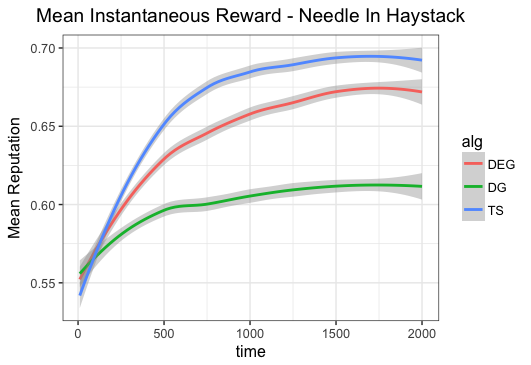
\includegraphics[scale=0.35]{ec19paper/appendix_figures/mean_inst_reward_nih}
\end{center}
\begin{center}
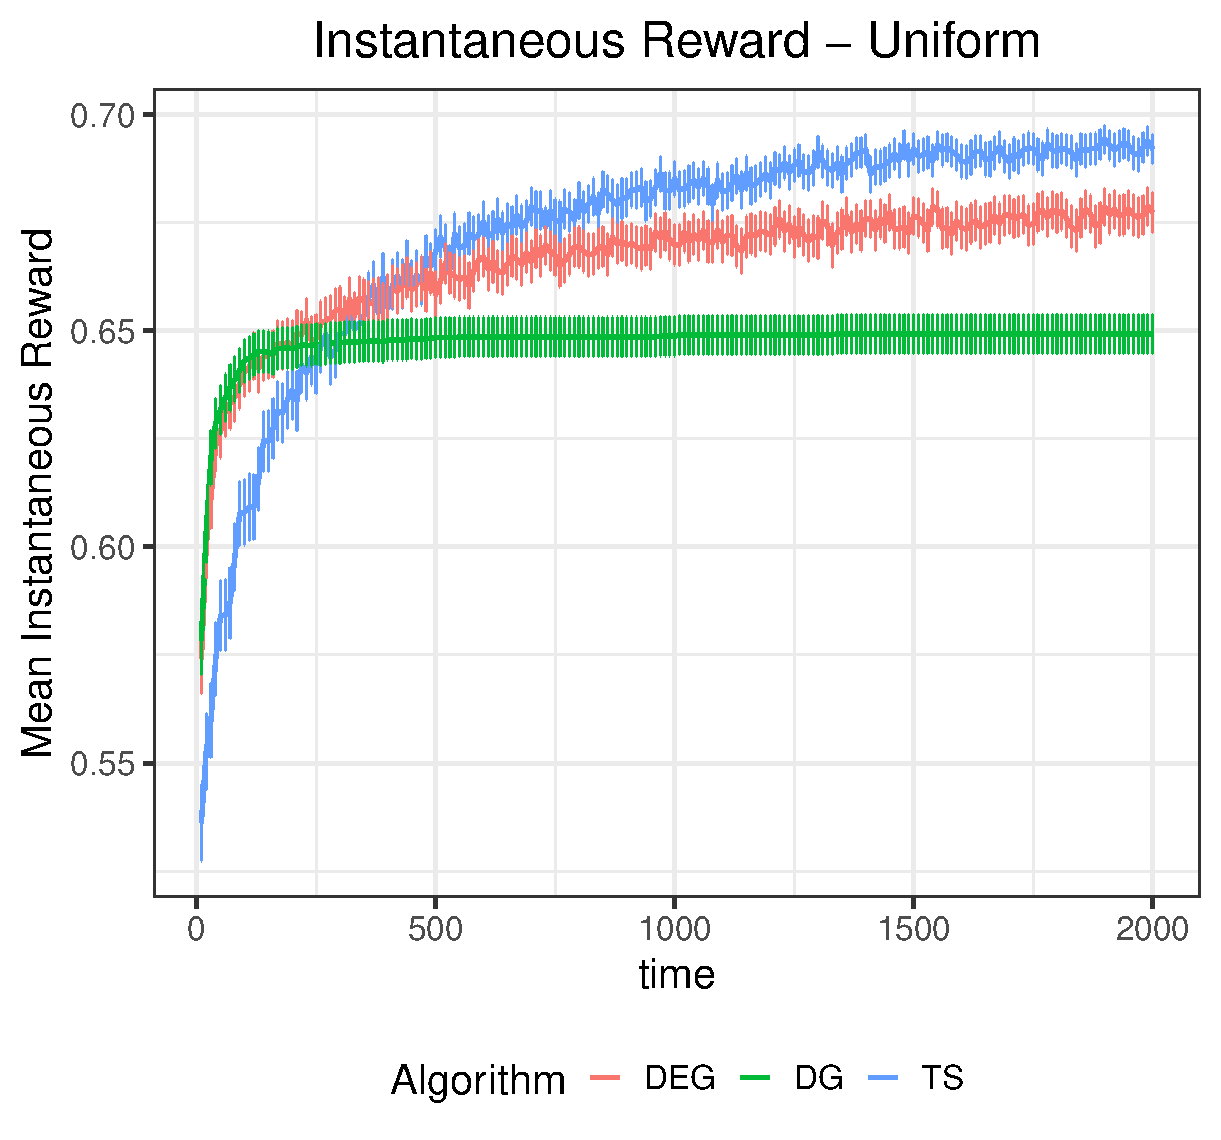
\includegraphics[scale=0.35]{ec19paper/appendix_figures/mean_inst_reward_uniform}
\end{center}

\subsection{Temporary Monopoly}

We present additional experiments on temporary monopoly from Section \ref{sec:competition}, across various MAB instances and various values of the incumbent advantage parameter $X$.

Each experiment is presented as a table with the same semantics as in the main text. Namely, each cell in the table describes the duopoly game between the entrant's algorithm (the row) and the incumbent's algorithm (the column). The cell specifies the entrant's market share (fraction of rounds in which it was chosen) for the rounds in which he was present. We give the average (in bold) and the 95\% confidence interval. NB: smaller average is better for the incumbent.

\OMIT{These results confirm the claim in the text that, for sufficiently large $X$, $\TS$ is preferred over all other algorithms for the incumbent. However, it also shows that, for smaller values of $X$ it is not necessarily the case that $\TS$ is the preferred algorithm. We provide many different parameterizations in order to check the robustness of the results. The interpretation of the tables is the same as those in the main text. The results presented here use the same instances and realization tables as those presented in the main text.}

\
\begin{table}[H]
\centering
\begin{tabular}{|c|c|c|c||c|c|c|}
  \hline
  & \multicolumn{3}{c||}{$X = 50$}
  & \multicolumn{3}{c|}{$X = 200$} \\
    \hline
  & $\TS$  & $\DEG$  & $\DG$
  & $\TS$  & $\DEG$  & $\DG$ \\
  \hline
  $\TS$
 & \makecell{\textbf{0.054} $\pm$0.01}
    & \makecell{\textbf{0.16} $\pm$0.02}
    & \makecell{\textbf{0.18} $\pm$0.02}
    %%
     & \makecell{\textbf{0.003} $\pm$0.003}
    & \makecell{\textbf{0.083} $\pm$0.02}
    & \makecell{\textbf{0.17} $\pm$0.02} \\\hline
    $\DEG$
    & \makecell{\textbf{0.33} $\pm$0.03}
    & \makecell{\textbf{0.31} $\pm$0.02}
    & \makecell{\textbf{0.26} $\pm$0.02}
    %%
    & \makecell{\textbf{0.045} $\pm$0.01}
    & \makecell{\textbf{0.25} $\pm$0.02}
    & \makecell{\textbf{0.23} $\pm$0.02} \\\hline
    $\DG$
    & \makecell{\textbf{0.39} $\pm$0.03}
    & \makecell{\textbf{0.41} $\pm$0.03}
    & \makecell{\textbf{0.33} $\pm$0.02}
    %%
    & \makecell{\textbf{0.12} $\pm$0.02}
    & \makecell{\textbf{0.36} $\pm$0.03}
    & \makecell{\textbf{0.3} $\pm$0.02} \\\hline
\end{tabular}
\caption{Heavy-Tail MAB Instance}
\end{table}


\scalebox{1.0}{\parbox{\linewidth}{%
\begin{table}[H]
\centering
\begin{tabular}{|c|c|c|c||c|c|c|}
  \hline
  & \multicolumn{3}{c||}{$X = 300$}
  & \multicolumn{3}{c|}{$X = 500$} \\
    \hline
  & $\TS$  & $\DEG$  & $\DG$
  & $\TS$  & $\DEG$  & $\DG$ \\
  \hline
  $\TS$
 & \makecell{\textbf{0.0017} $\pm$0.002}
    & \makecell{\textbf{0.059} $\pm$0.01}
    & \makecell{\textbf{0.16} $\pm$0.02}
    %%
       & \makecell{\textbf{0.002} $\pm$0.003}
    & \makecell{\textbf{0.043} $\pm$0.01}
    & \makecell{\textbf{0.16} $\pm$0.02} \\\hline
    $\DEG$
        & \makecell{\textbf{0.029} $\pm$0.007}
    & \makecell{\textbf{0.23} $\pm$0.02}
    & \makecell{\textbf{0.23} $\pm$0.02}
    %%
     & \makecell{\textbf{0.03} $\pm$0.007}
    & \makecell{\textbf{0.21} $\pm$0.02}
    & \makecell{\textbf{0.24} $\pm$0.02} \\\hline
    $\DG$
    & \makecell{\textbf{0.097} $\pm$0.02}
    & \makecell{\textbf{0.34} $\pm$0.03}
    & \makecell{\textbf{0.29} $\pm$0.02}
    %%
    & \makecell{\textbf{0.091} $\pm$0.01}
    & \makecell{\textbf{0.32} $\pm$0.03}
    & \makecell{\textbf{0.3} $\pm$0.02}\\\hline
\end{tabular}
\caption{Heavy-Tail MAB Instance}
\end{table}
}}


\begin{table}[H]
\centering
\begin{tabular}{|c|c|c|c||c|c|c|}
  \hline
  & \multicolumn{3}{c||}{$X = 50$}
  & \multicolumn{3}{c|}{$X = 200$} \\
    \hline
  & $\TS$  & $\DEG$  & $\DG$
  & $\TS$  & $\DEG$  & $\DG$ \\
  \hline
  $\TS$
 & \makecell{\textbf{0.34} $\pm$0.03}
    & \makecell{\textbf{0.4} $\pm$0.03}
    & \makecell{\textbf{0.48} $\pm$0.03}
    %%
      & \makecell{\textbf{0.17} $\pm$0.02}
    & \makecell{\textbf{0.31} $\pm$0.03}
    & \makecell{\textbf{0.41} $\pm$0.03} \\\hline
    $\DEG$
    & \makecell{\textbf{0.22} $\pm$0.02}
    & \makecell{\textbf{0.34} $\pm$0.03}
    & \makecell{\textbf{0.42} $\pm$0.03}
    %%
    & \makecell{\textbf{0.13} $\pm$0.02}
    & \makecell{\textbf{0.26} $\pm$0.02}
    & \makecell{\textbf{0.36} $\pm$0.03} \\\hline
    $\DG$
     & \makecell{\textbf{0.18} $\pm$0.02}
    & \makecell{\textbf{0.28} $\pm$0.02}
    & \makecell{\textbf{0.37} $\pm$0.03}
    %%
    & \makecell{\textbf{0.093} $\pm$0.02}
    & \makecell{\textbf{0.23} $\pm$0.02}
    & \makecell{\textbf{0.33} $\pm$0.03} \\\hline
\end{tabular}
\caption{Needle In Haystack MAB Instance}
\end{table}


\begin{table}[H]
\centering
\begin{tabular}{|c|c|c|c||c|c|c|}
  \hline
  & \multicolumn{3}{c||}{$X = 300$}
  & \multicolumn{3}{c|}{$X = 500$} \\
    \hline
  & $\TS$  & $\DEG$  & $\DG$
  & $\TS$  & $\DEG$  & $\DG$ \\
  \hline
  $\TS$
  & \makecell{\textbf{0.1} $\pm$0.02}
    & \makecell{\textbf{0.28} $\pm$0.03}
    & \makecell{\textbf{0.39} $\pm$0.03}
    %%
      & \makecell{\textbf{0.053} $\pm$0.01}
    & \makecell{\textbf{0.23} $\pm$0.02}
    & \makecell{\textbf{0.37} $\pm$0.03} \\\hline
    $\DEG$
         & \makecell{\textbf{0.089} $\pm$0.02}
    & \makecell{\textbf{0.23} $\pm$0.02}
    & \makecell{\textbf{0.36} $\pm$0.03}
    %%
      & \makecell{\textbf{0.051} $\pm$0.01}
    & \makecell{\textbf{0.2} $\pm$0.02}
    & \makecell{\textbf{0.33} $\pm$0.03} \\\hline
    $\DG$
     & \makecell{\textbf{0.05} $\pm$0.01}
    & \makecell{\textbf{0.21} $\pm$0.02}
    & \makecell{\textbf{0.33} $\pm$0.03}
    %%
    & \makecell{\textbf{0.031} $\pm$0.009}
    & \makecell{\textbf{0.18} $\pm$0.02}
    & \makecell{\textbf{0.31} $\pm$0.02} \\\hline
\end{tabular}
\caption{Needle In Haystack MAB Instance}
\end{table}

\begin{table}[H]
\centering
\begin{tabular}{|c|c|c|c||c|c|c|}
  \hline
  & \multicolumn{3}{c||}{$X = 50$}
  & \multicolumn{3}{c|}{$X = 200$} \\
    \hline
  & $\TS$  & $\DEG$  & $\DG$
  & $\TS$  & $\DEG$  & $\DG$ \\
  \hline
  $\TS$
  & \makecell{\textbf{0.27} $\pm$0.03}
    & \makecell{\textbf{0.21} $\pm$0.02}
    & \makecell{\textbf{0.26} $\pm$0.02}
    %%
   & \makecell{\textbf{0.12} $\pm$0.02}
    & \makecell{\textbf{0.16} $\pm$0.02}
    & \makecell{\textbf{0.2} $\pm$0.02} \\\hline
    $\DEG$
     & \makecell{\textbf{0.39} $\pm$0.03}
    & \makecell{\textbf{0.3} $\pm$0.03}
    & \makecell{\textbf{0.34} $\pm$0.03}
    %%
     & \makecell{\textbf{0.25} $\pm$0.02}
    & \makecell{\textbf{0.24} $\pm$0.02}
    & \makecell{\textbf{0.29} $\pm$0.02} \\\hline
    $\DG$
     & \makecell{\textbf{0.39} $\pm$0.03}
    & \makecell{\textbf{0.31} $\pm$0.02}
    & \makecell{\textbf{0.33} $\pm$0.02}
    %%
    & \makecell{\textbf{0.23} $\pm$0.02}
    & \makecell{\textbf{0.24} $\pm$0.02}
    & \makecell{\textbf{0.29} $\pm$0.02} \\\hline
\end{tabular}
\caption{Uniform MAB Instance}
\end{table}


\begin{table}[H]
\centering
\begin{tabular}{|c|c|c|c||c|c|c|}
  \hline
  & \multicolumn{3}{c||}{$X = 300$}
  & \multicolumn{3}{c|}{$X = 500$} \\
    \hline
  & $\TS$  & $\DEG$  & $\DG$
  & $\TS$  & $\DEG$  & $\DG$ \\
  \hline
  $\TS$
  & \makecell{\textbf{0.094} $\pm$0.02}
    & \makecell{\textbf{0.15} $\pm$0.02}
    & \makecell{\textbf{0.2} $\pm$0.02}
    %%
     & \makecell{\textbf{0.061} $\pm$0.01}
    & \makecell{\textbf{0.12} $\pm$0.02}
    & \makecell{\textbf{0.2} $\pm$0.02} \\\hline
    $\DEG$
      & \makecell{\textbf{0.2} $\pm$0.02}
    & \makecell{\textbf{0.23} $\pm$0.02}
    & \makecell{\textbf{0.29} $\pm$0.02}
    %%
     & \makecell{\textbf{0.17} $\pm$0.02}
    & \makecell{\textbf{0.21} $\pm$0.02}
    & \makecell{\textbf{0.29} $\pm$0.02} \\\hline
    $\DG$
  & \makecell{\textbf{0.21} $\pm$0.02}
    & \makecell{\textbf{0.23} $\pm$0.02}
    & \makecell{\textbf{0.29} $\pm$0.02}
    %%
  & \makecell{\textbf{0.18} $\pm$0.02}
    & \makecell{\textbf{0.22} $\pm$0.02}
    & \makecell{\textbf{0.29} $\pm$0.02} \\\hline
\end{tabular}
\caption{Uniform MAB Instance}
\end{table}

\subsection{Reputation vs. Data Advantage}

This section presents all experiments on data vs. reputation advantage (Section \ref{sec:barriers}).

Each experiment is presented as a table with the same semantics as in the main text. Namely, each cell in the table describes the duopoly game between the entrant's algorithm (the {\bf row}) and the incumbent's algorithm (the {\bf column}). The cell specifies the entrant's market share for the rounds in which hit was present: the average (in bold) and the 95\% confidence interval. NB: smaller average is better for the incumbent.



\begin{table}[H]
\centering
\begin{tabular}{|c|c|c|c||c|c|c|}
  \hline
  & \multicolumn{3}{c||}{Data Advantage}
  & \multicolumn{3}{c|}{Reputation Advantage} \\
    \hline
  & $\TS$  & $\DEG$  & $\DG$
  & $\TS$  & $\DEG$  & $\DG$ \\
  \hline
  $\TS$
   & \makecell{\textbf{ 0.0096 } $\pm$ 0.006}
    & \makecell{\textbf{ 0.11 } $\pm$ 0.02}
    & \makecell{\textbf{ 0.18 } $\pm$ 0.02}
    %%
       & \makecell{\textbf{ 0.021 } $\pm$ 0.009}
    & \makecell{\textbf{ 0.16 } $\pm$ 0.02}
    & \makecell{\textbf{ 0.21 } $\pm$ 0.02} \\\hline
    $\DEG$
     & \makecell{\textbf{ 0.073 } $\pm$ 0.01}
    & \makecell{\textbf{ 0.29 } $\pm$ 0.02}
    & \makecell{\textbf{ 0.25 } $\pm$ 0.02}
    %%
     & \makecell{\textbf{ 0.26 } $\pm$ 0.03}
    & \makecell{\textbf{ 0.3 } $\pm$ 0.02}
    & \makecell{\textbf{ 0.26 } $\pm$ 0.02} \\\hline
    $\DG$
   & \makecell{\textbf{ 0.15 } $\pm$ 0.02}
    & \makecell{\textbf{ 0.39 } $\pm$ 0.03}
    & \makecell{\textbf{ 0.33 } $\pm$ 0.02}
    %%
   & \makecell{\textbf{ 0.34 } $\pm$ 0.03}
    & \makecell{\textbf{ 0.4 } $\pm$ 0.03 }
    & \makecell{\textbf{ 0.33 } $\pm$ 0.02} \\\hline
\end{tabular}
\caption{Heavy Tail MAB Instance, $X = 200$}
\end{table}


\begin{table}[H]
\centering
\begin{tabular}{|c|c|c|c||c|c|c|}
  \hline
  & \multicolumn{3}{c||}{Data Advantage}
  & \multicolumn{3}{c|}{Reputation Advantage} \\
    \hline
  & $\TS$  & $\DEG$  & $\DG$
  & $\TS$  & $\DEG$  & $\DG$ \\
  \hline
  $\TS$
      & \makecell{\textbf{0.0017} $\pm$0.002}
    & \makecell{\textbf{0.06} $\pm$0.01}
    & \makecell{\textbf{0.18} $\pm$0.02}
    %%
    & \makecell{\textbf{0.022} $\pm$0.009}
    & \makecell{\textbf{0.13} $\pm$0.02}
    & \makecell{\textbf{0.21} $\pm$0.02} \\\hline
    $\DEG$
      & \makecell{\textbf{0.04} $\pm$0.009}
    & \makecell{\textbf{0.24} $\pm$0.02}
    & \makecell{\textbf{0.25} $\pm$0.02}
    %%
  & \makecell{\textbf{0.26} $\pm$0.03}
    & \makecell{\textbf{0.29} $\pm$0.02}
    & \makecell{\textbf{0.28} $\pm$0.02} \\\hline
    $\DG$
   & \makecell{\textbf{0.12} $\pm$0.02}
    & \makecell{\textbf{0.35} $\pm$0.03}
    & \makecell{\textbf{0.33} $\pm$0.02}
    %%
   & \makecell{\textbf{0.33} $\pm$0.03}
    & \makecell{\textbf{0.39} $\pm$0.03}
    & \makecell{\textbf{0.34} $\pm$0.02} \\\hline
\end{tabular}
\caption{Heavy Tail MAB Instance, $X = 500$}
\end{table}

\begin{table}[H]
\centering
\begin{tabular}{|c|c|c|c||c|c|c|}
  \hline
  & \multicolumn{3}{c||}{Data Advantage}
  & \multicolumn{3}{c|}{Reputation Advantage} \\
    \hline
  & $\TS$  & $\DEG$  & $\DG$
  & $\TS$  & $\DEG$  & $\DG$ \\
  \hline
  $\TS$
   & \makecell{\textbf{ 0.25 } $\pm$ 0.03}
    & \makecell{\textbf{ 0.36 } $\pm$ 0.03}
    & \makecell{\textbf{ 0.45 } $\pm$ 0.03}
    %%
     & \makecell{\textbf{ 0.35 } $\pm$ 0.03}
    & \makecell{\textbf{ 0.43 } $\pm$ 0.03}
    & \makecell{\textbf{ 0.52 } $\pm$ 0.03} \\\hline
    $\DEG$
    & \makecell{\textbf{ 0.21 } $\pm$ 0.02}
    & \makecell{\textbf{ 0.32 } $\pm$ 0.03}
    & \makecell{\textbf{ 0.41 } $\pm$ 0.03}
    %%
     & \makecell{\textbf{ 0.26 } $\pm$ 0.03 }
    & \makecell{\textbf{ 0.36 } $\pm$ 0.03}
    & \makecell{\textbf{ 0.43 } $\pm$ 0.03} \\\hline
    $\DG$
   & \makecell{\textbf{ 0.18 } $\pm$ 0.02}
    & \makecell{\textbf{ 0.29 } $\pm$ 0.03}
    & \makecell{\textbf{ 0.4 } $\pm$ 0.03}
    %%
    & \makecell{\textbf{ 0.19 } $\pm$ 0.02}
    & \makecell{\textbf{ 0.3 } $\pm$ 0.02}
    & \makecell{\textbf{ 0.36 } $\pm$ 0.02} \\\hline
\end{tabular}
\caption{Needle-in-Haystack MAB Instance, $X=200$}
\end{table}


\begin{table}[H]
\centering
\begin{tabular}{|c|c|c|c||c|c|c|}
  \hline
  & \multicolumn{3}{c||}{Data Advantage}
  & \multicolumn{3}{c|}{Reputation Advantage} \\
    \hline
  & $\TS$  & $\DEG$  & $\DG$
  & $\TS$  & $\DEG$  & $\DG$ \\
  \hline
  $\TS$
  & \makecell{\textbf{0.098} $\pm$0.02}
    & \makecell{\textbf{0.27} $\pm$0.03}
    & \makecell{\textbf{0.41} $\pm$0.03}
    %%
     & \makecell{\textbf{0.29} $\pm$0.03}
    & \makecell{\textbf{0.44} $\pm$0.03}
    & \makecell{\textbf{0.52} $\pm$0.03} \\\hline
    $\DEG$
      & \makecell{\textbf{0.093} $\pm$0.02}
    & \makecell{\textbf{0.24} $\pm$0.02}
    & \makecell{\textbf{0.38} $\pm$0.03}
    %%
    & \makecell{\textbf{0.19} $\pm$0.02}
    & \makecell{\textbf{0.35} $\pm$0.03}
    & \makecell{\textbf{0.42} $\pm$0.03} \\\hline
    $\DG$
    & \makecell{\textbf{0.064} $\pm$0.01}
    & \makecell{\textbf{0.22} $\pm$0.02}
    & \makecell{\textbf{0.37} $\pm$0.03}
    %%
    & \makecell{\textbf{0.15} $\pm$0.02}
    & \makecell{\textbf{0.27} $\pm$0.02}
    & \makecell{\textbf{0.35} $\pm$0.02} \\\hline
\end{tabular}
\caption{Needle-in-Haystack MAB Instance, $X=500$}
\end{table}


\begin{table}[H]
\centering
\begin{tabular}{|c|c|c|c||c|c|c|}
  \hline
  & \multicolumn{3}{c||}{Data Advantage}
  & \multicolumn{3}{c|}{Reputation Advantage} \\
    \hline
  & $\TS$  & $\DEG$  & $\DG$
  & $\TS$  & $\DEG$  & $\DG$ \\
  \hline
  $\TS$
  & \makecell{\textbf{ 0.2 } $\pm$ 0.02}
    & \makecell{\textbf{ 0.22 } $\pm$ 0.02}
    & \makecell{\textbf{ 0.27 } $\pm$ 0.03}
    %%
     & \makecell{\textbf{ 0.27 } $\pm$ 0.03}
    & \makecell{\textbf{ 0.23 } $\pm$ 0.02}
    & \makecell{\textbf{ 0.27 } $\pm$ 0.02}\\\hline
    $\DEG$
    & \makecell{\textbf{ 0.33 } $\pm$ 0.03}
    & \makecell{\textbf{ 0.32 } $\pm$ 0.03}
    & \makecell{\textbf{ 0.35 } $\pm$ 0.03}
    %%
     & \makecell{\textbf{ 0.4 } $\pm$ 0.03}
    & \makecell{\textbf{ 0.3 } $\pm$ 0.02 }
    & \makecell{\textbf{ 0.32 } $\pm$ 0.02} \\\hline
    $\DG$
    & \makecell{\textbf{ 0.32 } $\pm$ 0.03}
    & \makecell{\textbf{ 0.31 } $\pm$ 0.03}
    & \makecell{\textbf{ 0.35 } $\pm$ 0.03}
    %%
     & \makecell{\textbf{ 0.36 } $\pm$ 0.03}
    & \makecell{\textbf{ 0.29 } $\pm$ 0.02}
    & \makecell{\textbf{ 0.3 } $\pm$ 0.02} \\\hline
\end{tabular}
\caption{Uniform MAB Instance, $X = 200$}
\end{table}

\begin{table}[H]
\centering
\begin{tabular}{|c|c|c|c||c|c|c|}
  \hline
  & \multicolumn{3}{c||}{Data Advantage}
  & \multicolumn{3}{c|}{Reputation Advantage} \\
    \hline
  & $\TS$  & $\DEG$  & $\DG$
  & $\TS$  & $\DEG$  & $\DG$ \\
  \hline
  $\TS$
 & \makecell{\textbf{0.14} $\pm$0.02}
    & \makecell{\textbf{0.18} $\pm$0.02}
    & \makecell{\textbf{0.26} $\pm$0.03}
    %%
    & \makecell{\textbf{0.24} $\pm$0.02}
    & \makecell{\textbf{0.2} $\pm$0.02}
    & \makecell{\textbf{0.26} $\pm$0.02}\\\hline
    $\DEG$
  & \makecell{\textbf{0.26} $\pm$0.02}
    & \makecell{\textbf{0.26} $\pm$0.02}
    & \makecell{\textbf{0.34} $\pm$0.03}
    %%
   & \makecell{\textbf{0.37} $\pm$0.03}
    & \makecell{\textbf{0.29} $\pm$0.02}
    & \makecell{\textbf{0.31} $\pm$0.02} \\\hline
    $\DG$
    & \makecell{\textbf{0.25} $\pm$0.02}
    & \makecell{\textbf{0.27} $\pm$0.02}
    & \makecell{\textbf{0.34} $\pm$0.03}
    %%
     & \makecell{\textbf{0.35} $\pm$0.03}
    & \makecell{\textbf{0.27} $\pm$0.02}
    & \makecell{\textbf{0.3} $\pm$0.02}  \\\hline
\end{tabular}
\caption{Uniform MAB Instance, $X = 500$}
\end{table}

\subsection{Mean Reputation vs. Relative Reputation}

We present the experiments omitted from Section \ref{sec:revisited}. Namely, experiments on the Heavy-Tail MAB instance with $K=3$ arms, both for ``performance in isolation" and the permanent duopoly game. We find that $\DEG > \DG$ according to the mean reputation trajectory but that $\DG > \DEG$ according to the relative reputation trajectory \emph{and} in the competition game. As discussed in Section \ref{sec:revisited}, the same results also hold for $K = 10$ for the warm starts that we consider.

The result of the permanent duopoly experiment for this instance  is shown in Table \ref{ht_k3}.

\begin{table}[h]
\centering
\begin{tabular}{|c|c|c|c|}
  \hline
  & \multicolumn{3}{c|}{Heavy-Tail} \\
\hline
   & $T_0$ = 20 & $T_0$ = 250 & $T_0$ = 500 \\ \hline
\TS vs. \DG
  & \makecell{\textbf{0.4} $\pm$0.02\\ \Eeog 770 (0)}
    & \makecell{\textbf{0.59} $\pm$0.01\\ \Eeog 2700 (2979.5)}
    & \makecell{\textbf{0.6} $\pm$0.01\\ \Eeog 2700 (3018)} \\ \hline
\TS vs. \DEG
    & \makecell{\textbf{0.46} $\pm$0.02 \\ \Eeog 830 (0)}
    & \makecell{\textbf{0.73} $\pm$0.01 \\ \Eeog 2500 (2576.5)}
    & \makecell{\textbf{0.72} $\pm$0.01 \\ \Eeog 2700 (2862)} \\ \hline
\DG vs. \DEG
    & \makecell{\textbf{0.61} $\pm$0.01 \\ \Eeog 1400 (556)}
    & \makecell{\textbf{0.61} $\pm$0.01 \\ \Eeog 2400 (2538.5)}
    & \makecell{\textbf{0.6} $\pm$0.01 \\ \Eeog 2400 (2587.5)} \\\hline
\end{tabular}
\caption{Duopoly Experiment: Heavy-Tail, $K=3$, $T=5000$.\\
Each cell describes a game between two algorithms, call them Alg1 vs. Alg2, for a particular value of the warm start $T_0$. Line 1 in the cell is the market share of Alg 1: the average (in bold) and the 95\% confidence band.
%For example, the cell in the top left indicates that TS gets on average 64\% of the market when played against DG.
Line 2 specifies the ``effective end of game" (\Eeog): the average and the median (in brackets). }
\label{ht_k3}
\end{table}

The mean reputation trajectories for algorithms' performance in isolation:
\begin{center}
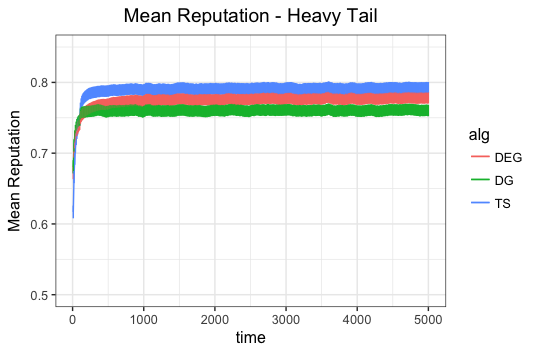
\includegraphics[scale=0.35]{ec19paper/appendix_figures/mean_ht_3_arms} \\
\end{center}

Finally, the relative reputation trajectory of \DEG vs. \DG:
\begin{center}
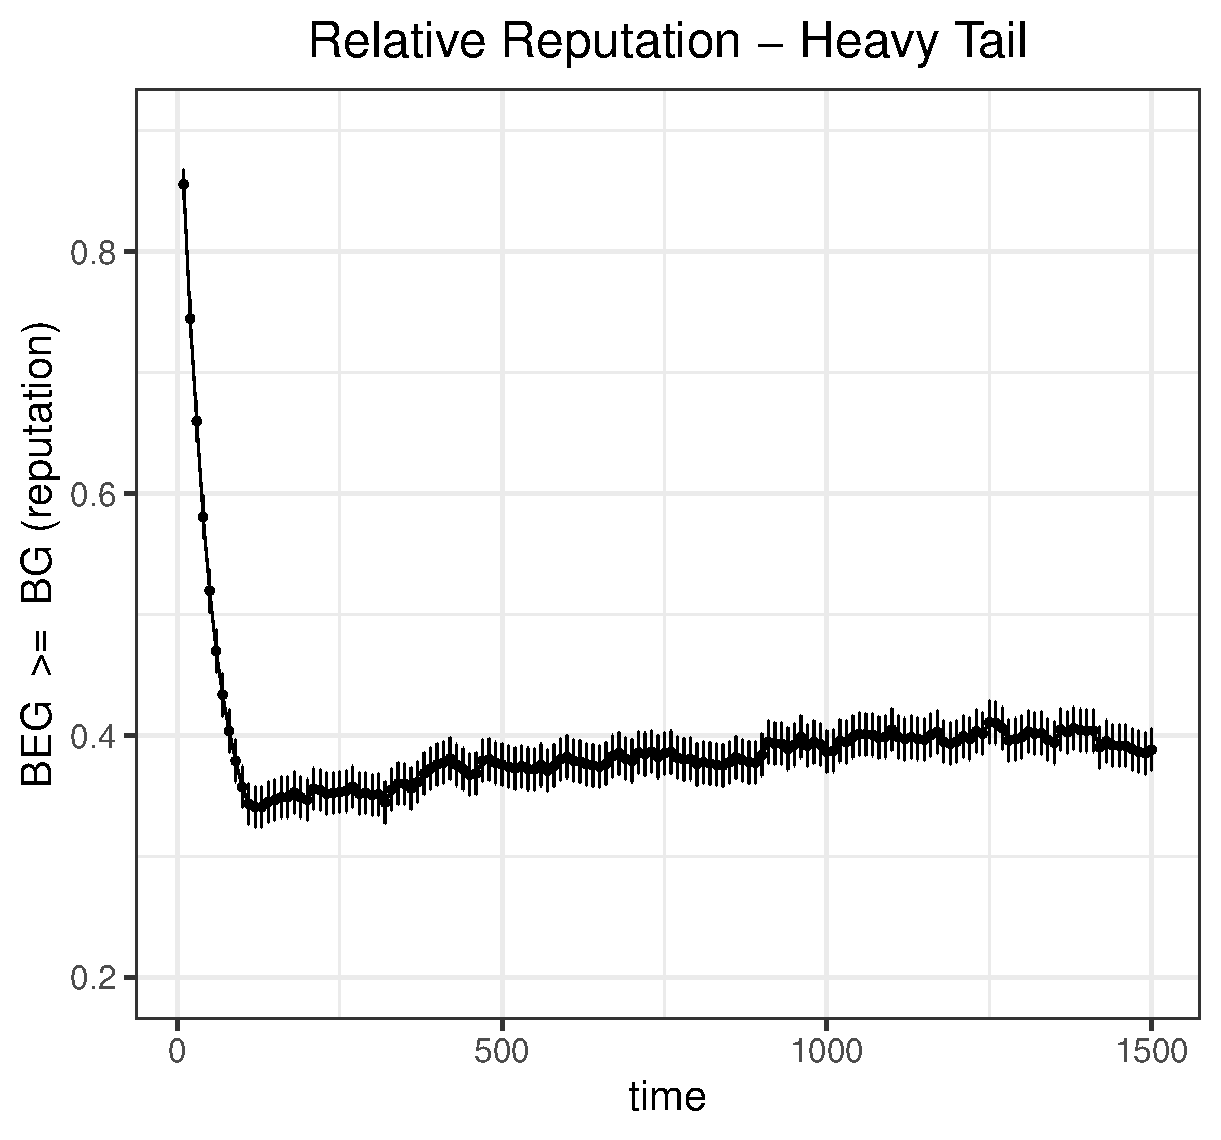
\includegraphics[scale=0.35]{ec19paper/appendix_figures/rel_rep_ht_3_arms}
\end{center}


\end{document}
